\documentclass{beamer}
%
% Choose how your presentation looks.
%
% For more themes, color themes and font themes, see:
% http://deic.uab.es/~iblanes/beamer_gallery/index_by_theme.html
%
\mode<presentation>
{
  \usetheme{default}      % or try Darmstadt, Madrid, Warsaw, ...
  \usecolortheme{default} % or try albatross, beaver, crane, ...
  \usefonttheme{default}  % or try serif, structurebold, ...
  \setbeamertemplate{navigation symbols}{}
  \setbeamertemplate{caption}[numbered]
} 

\usepackage[english]{babel}
\usepackage[utf8x]{inputenc}

\title[Your Short Title]{Protein-Protein Binding Affinity}
\author{Alen Aliev}
\institute{MIPT}
\date{}

\begin{document}

\begin{frame}
  \titlepage
\end{frame}

% Uncomment these lines for an automatically generated outline.
%\begin{frame}{Outline}
%  \tableofcontents
%\end{frame}

\section{Some \LaTeX{} Examples}

\subsection{Protein Interaction Problem}

\begin{frame}{Protein-Protein Binding Affinity}

We analyze protein complexes interactions. \\ 
\bigskip

Our goal is to provide a model for predicting binding affinity of complexes. \\
\bigskip

We suggest using deep-learning methods, i.e. Graph Neural Networks and CNN.

\end{frame}


\begin{frame}{Protein Interaction Problem}

% Commands to include a figure:
\begin{figure}
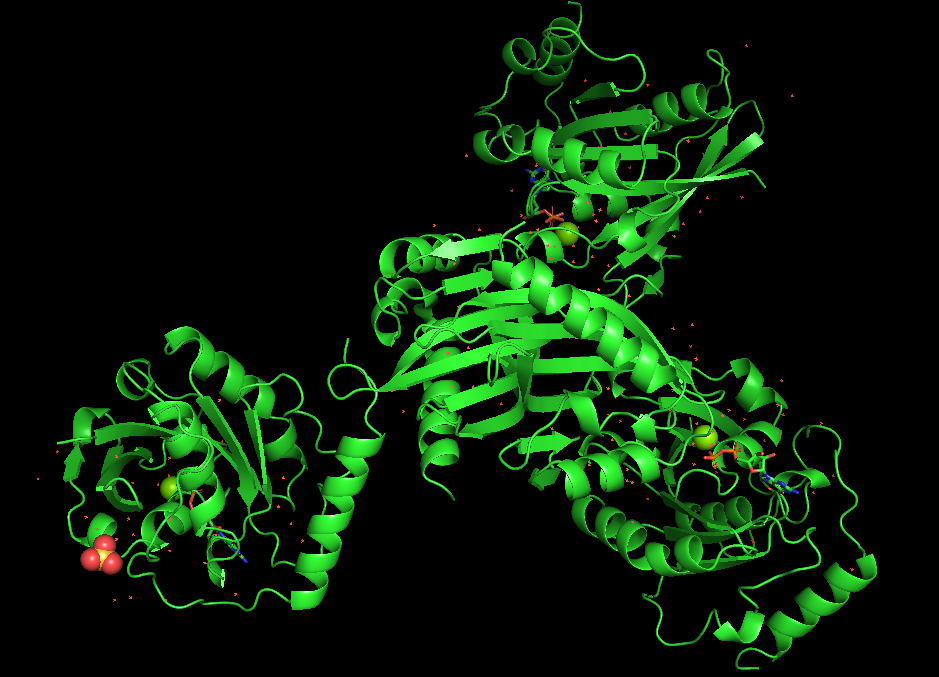
\includegraphics[width=200px, height=140px]{ProteinExample.png}
\caption{\label{fig:your-figure}Protein Complex Example}
\end{figure}

$\mathcal{A} = \{Ala, Arg, Asn, \ldots, Val \}$ \\
$a_i \in \mathbf{R}^3$ - atom \\
$PR = \{a_i\} \in  {\mathbf{R}^3}^*$ - single protein \\
$PC = (PR_0, PR_1)$ - protein complex \\

\end{frame}


\begin{frame}{Literature}
\begin{itemize}
        \item K Yugandhar and M Michael Gromiha. Computational approaches for predicting binding partners, interface residues, and binding affinity of protein–protein complexes. Springer, 2017 
        \item Anna Vangone and Alexandre MJJ Bonvin. Contacts-based prediction of binding affinity in protein–protein complexes, 2015. 
        \item Iain H Moal, Rudi Agius, and Paul A Bates. Protein–protein binding affinity prediction on a diverse set of structures. Bioinformatics, 2011.
\end{itemize}
\end{frame}

\begin{frame}{Protein Dataset Description}
Dataset consists of protein chains, taken from pdbbind.org
\bigskip

Our hypothesis is that the interacting atoms are the ones selected with KNN method.
\bigskip

Two chains are considered interacting if they maximize number of atoms-neighbours.
\end{frame}

\begin{frame}{Affinity Prediction Analysis}
\begin{figure}
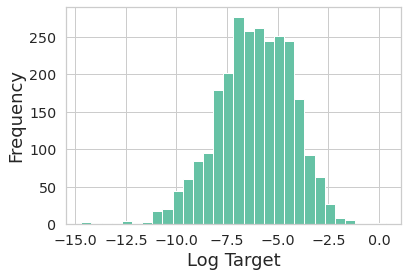
\includegraphics[width=200px, height=140px]{logM.png}
\caption{\label{fig:your-figure}Log of Target Distribution}
\end{figure}

We predict logarithm of target.

We benchmark models against existing state-of-the-art solutions using MSE metric and batch accuracy.
\end{frame}

\begin{frame}{Problem Solution: 3D grid}
We define $C_{PR_0, PR_1}$ as center of mass of all interacting atoms in chains.
\bigskip

Each complex is now a 3D grid centered around $C_{PR_0, PR_1}$.
\bigskip

This grid is used with 3D CNN.
\end{frame}

\begin{frame}{Problem Solution: Graph}
Let $\mathsf{V} = PR_0 \cup PR_1$
\bigskip

We say that $(a_i, a_j) \in \mathsf{E} \leftrightarrow a_j$ is in K Nearest Neighbours of $a_i$.
\bigskip

This graph $G = (V, E)$ representation is used with Graph Neural Network.
\end{frame}

\begin{frame}{Computational Experiment}

\begin{figure}
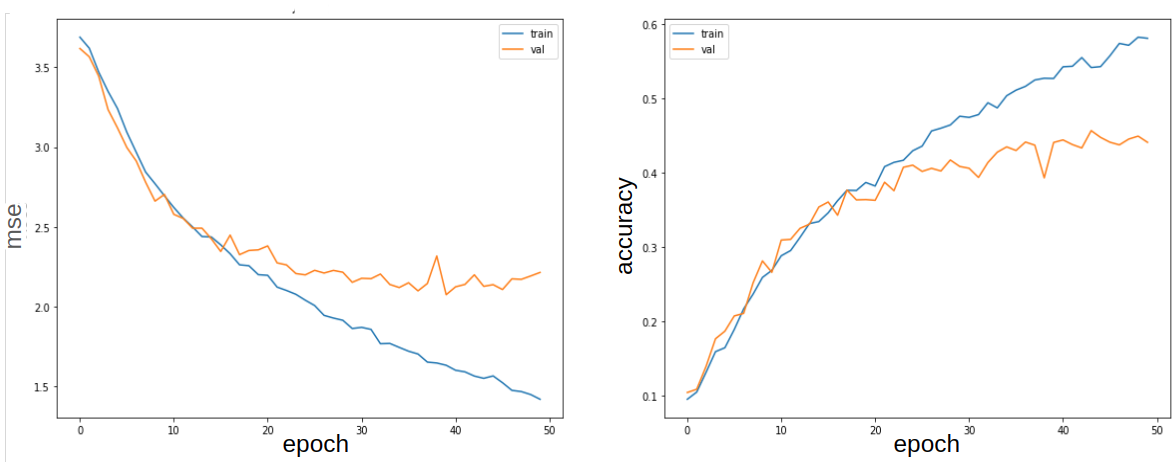
\includegraphics[width=280px, height=140px]{CNN_error.png}
\caption{\label{fig:your-figure}CNN performance}
\end{figure}

Around 50 epochs is sufficient to fit the model according to stoppage criterion.
\end{frame}

\begin{frame}{Error Analysis}
\begin{tabular}{ |p{4cm}|p{3cm}|p{3cm}|  }
    \hline
    \multicolumn{3}{|c|}{Test metrics} \\
    \hline
    Model & MSE & Accuracy\\
    \hline
    3D-CNN, VGG based & 0.8715 & 0.72\\
    Graph NN & 0.9 & 0.71 \\
    CatBoost & 1.2 & 0.53\\
    Basic Model & 4.8 & 0.172\\
    \hline
\end{tabular}
\end{frame}

\begin{frame}{Conclusion}
\begin{itemize}
    \item We provide two different interpretations of protein complex
    \item Implemented the model for predicting affinity of PPB.
\end{itemize}
\textbf{Next:} hyperparameters fitting. 
\end{frame}

\end{document}
